% vim: set spell spelllang=en tw=100 et sw=4 sts=4 foldmethod=marker foldmarker={{{,}}} :

\documentclass[aspectratio=169,compress,10pt]{beamer}

\usepackage{tikz}
\usepackage{xcolor}
\usepackage{complexity}
\usepackage{hyperref}
\usepackage{microtype}
\usepackage{amsmath}                   % \operatorname
\usepackage{amsfonts}                  % \mathcal
\usepackage{amssymb}                   % \nexists
\usepackage[vlined]{algorithm2e} % algorithms
\usepackage{centernot}
\usepackage{listings}
\usepackage{csquotes}
\usepackage{fancyvrb}
\usepackage{bussproofs}
\usepackage{multicol}
\usepackage{booktabs}
\usepackage{mathtools}
\usepackage{pifont}
\usepackage{marvosym}
\usepackage{cancel}

\usefonttheme{professionalfonts}

\usetikzlibrary{shapes, arrows, shadows, calc, positioning, fit}
\usetikzlibrary{decorations.pathreplacing, decorations.pathmorphing, shapes.misc}
\usetikzlibrary{tikzmark, backgrounds}
\usetikzlibrary{trees, overlay-beamer-styles}

\tikzset{processarrow/.style={->, very thick, decorate, decoration={snake, post length=0.5mm}}}
\tikzset{brace/.style={decorate, decoration={brace}, very thick}}

\definecolor{uofguniversityblue}{rgb}{0, 0.219608, 0.396078}
\definecolor{uofgheather}{rgb}{0.356863, 0.32549, 0.490196}
\definecolor{uofgaquamarine}{rgb}{0.603922, 0.72549, 0.678431}
\definecolor{uofgslate}{rgb}{0.309804, 0.34902, 0.380392}
\definecolor{uofgrose}{rgb}{0.823529, 0.470588, 0.709804}
\definecolor{uofgmocha}{rgb}{0.709804, 0.564706, 0.47451}
\definecolor{uofgsandstone}{rgb}{0.321569, 0.278431, 0.231373}
\definecolor{uofgforest}{rgb}{0, 0.2, 0.129412}
\definecolor{uofglawn}{rgb}{0.517647, 0.741176, 0}
\definecolor{uofgcobalt}{rgb}{0, 0.615686, 0.92549}
\definecolor{uofgturquoise}{rgb}{0, 0.709804, 0.819608}
\definecolor{uofgsunshine}{rgb}{1.0, 0.862745, 0.211765}
\definecolor{uofgpumpkin}{rgb}{1.0, 0.72549, 0.282353}
\definecolor{uofgthistle}{rgb}{0.584314, 0.070588, 0.447059}
\definecolor{uofgrust}{rgb}{0.603922, 0.227451, 0.023529}
\definecolor{uofgburgundy}{rgb}{0.490196, 0.133333, 0.223529}
\definecolor{uofgpillarbox}{rgb}{0.701961, 0.047059, 0}
\definecolor{uofglavendar}{rgb}{0.356863, 0.301961, 0.580392}

% {{{ theme things
\useoutertheme[footline=authortitle]{miniframes}
\useinnertheme{rectangles}

\setbeamerfont{block title}{size={}}
\setbeamerfont{title}{size=\large,series=\bfseries}
\setbeamerfont{section title}{size=\large,series=\mdseries}
\setbeamerfont{author}{size=\normalsize,series=\mdseries}
\setbeamercolor*{structure}{fg=uofguniversityblue}
\setbeamercolor*{palette primary}{use=structure,fg=black,bg=white}
\setbeamercolor*{palette secondary}{use=structure,fg=white,bg=uofgcobalt}
\setbeamercolor*{palette tertiary}{use=structure,fg=white,bg=uofguniversityblue}
\setbeamercolor*{palette quaternary}{fg=white,bg=black}
\setbeamercolor{block body}{bg=structure!10}
\setbeamercolor{block title}{bg=structure,fg=white}
\setbeamertemplate{blocks}[rounded]
\setbeamercolor*{titlelike}{parent=palette primary}

\beamertemplatenavigationsymbolsempty

\setbeamertemplate{title page}
{
    \begin{tikzpicture}[remember picture, overlay]
        \node at (current page.north west) {
            \begin{tikzpicture}[remember picture, overlay]
                \fill [fill=uofguniversityblue, anchor=north west] (0, 0) rectangle (\paperwidth, -2.6cm);
            \end{tikzpicture}
        };

        \node (logo) [anchor=north east, shift={(-0.8cm,-0.2cm)}] at (current page.north east) {
            
\includegraphics[keepaspectratio=true,scale=0.5]{../../images/UoG_keyline.pdf}
        };

        \node (logo2) [anchor=north, below=0.2cm of logo.south] {
            
\includegraphics[keepaspectratio=true,scale=0.1]{../../images/RAEngWhite.pdf}
        };

        \coordinate (logos) at ($(logo.south)!0.5!(logo2.north)$);

        \node [anchor=west, xshift=0.8cm] at (current page.west |- logos) {
            \begin{minipage}{0.65\paperwidth}\raggedright
                {\usebeamerfont{title}\usebeamercolor[white]{}\inserttitle}\\[0.1cm]
                {\usebeamerfont{author}\usebeamercolor[white]{}\insertauthor}
            \end{minipage}
        };
    \end{tikzpicture}
}

\setbeamertemplate{section page}
{
    \begin{centering}
        \begin{beamercolorbox}[sep=12pt,center]{part title}
            \usebeamerfont{section title}\insertsection\par
        \end{beamercolorbox}
    \end{centering}
}

\newcommand{\frameofframes}{/}
\newcommand{\setframeofframes}[1]{\renewcommand{\frameofframes}{#1}}

\makeatletter
\setbeamertemplate{footline}
{%
    \begin{beamercolorbox}[colsep=1.5pt]{upper separation line foot}
    \end{beamercolorbox}
    \begin{beamercolorbox}[ht=2.5ex,dp=1.125ex,%
        leftskip=.3cm,rightskip=.3cm plus1fil]{author in head/foot}%
        \leavevmode{\usebeamerfont{author in head/foot}\insertshortauthor}%
        \hfill%
        {\usebeamerfont{institute in head/foot}\usebeamercolor[fg]{institute in head/foot}\insertshortinstitute}%
    \end{beamercolorbox}%
    \begin{beamercolorbox}[ht=2.5ex,dp=1.125ex,%
        leftskip=.3cm,rightskip=.3cm plus1fil]{title in head/foot}%
        {\usebeamerfont{title in head/foot}\insertshorttitle}%
        \hfill%
        {\usebeamerfont{frame number}\usebeamercolor[fg]{frame number}\insertframenumber~\frameofframes~\inserttotalframenumber}
    \end{beamercolorbox}%
    \begin{beamercolorbox}[colsep=1.5pt]{lower separation line foot}
    \end{beamercolorbox}
}

\makeatletter
\setbeamertemplate{mini frame}
{%
  \begin{pgfpicture}{0pt}{0pt}{.04cm}{.04cm}
    \pgfpathcircle{\pgfpoint{0.04cm}{0.04cm}}{0.04cm}
    \pgfusepath{fill,stroke}
  \end{pgfpicture}%
}
\setbeamertemplate{mini frame in current subsection}
{%
  \begin{pgfpicture}{0pt}{0pt}{.04cm}{.04cm}
    \pgfpathcircle{\pgfpoint{0.04cm}{0.04cm}}{0.04cm}
    \pgfsetfillcolor{section in head/foot.bg}
    \pgfusepath{fill,stroke}
  \end{pgfpicture}%
}

\setbeamersize{mini frame size=0.10cm, mini frame offset=0.06cm}
\makeatother

% }}}

\author{Ciaran McCreesh}
\title{Fellowships}

\begin{document}

{
    \usebackgroundtemplate{
        \tikz[overlay, remember picture]
        \node[at=(current page.south), anchor=south, inner sep=0pt, yshift=-1.4cm]{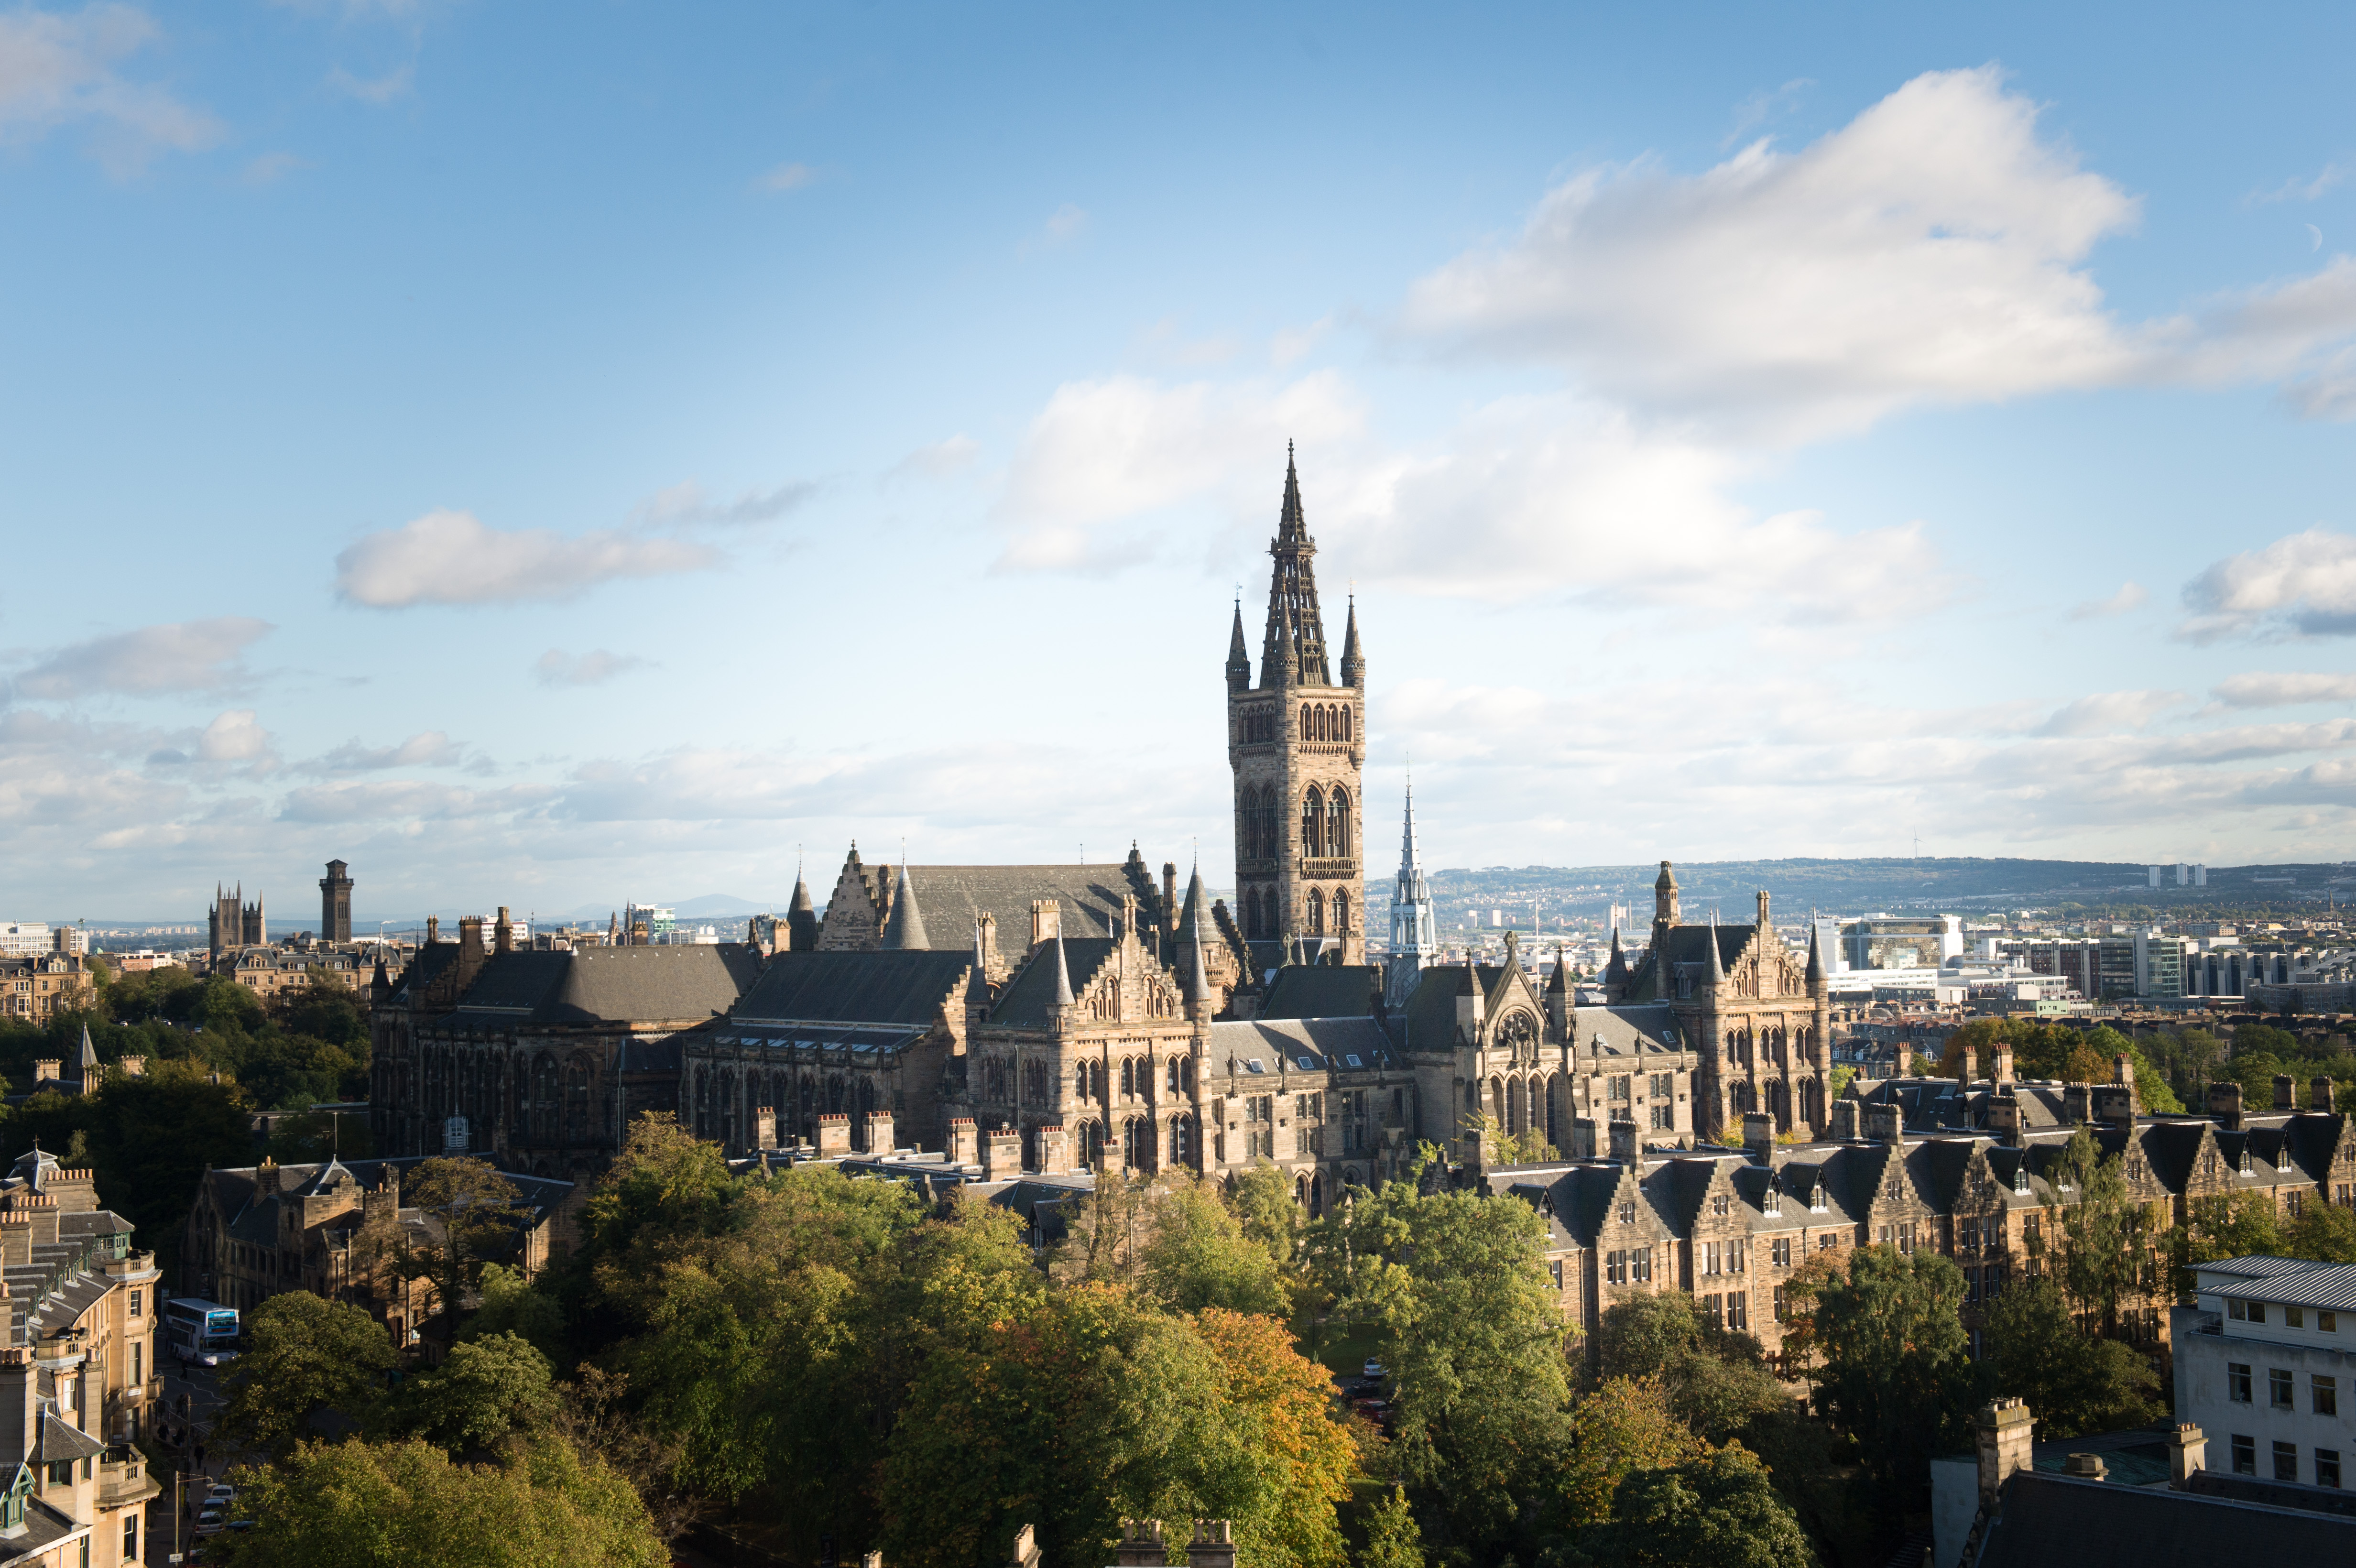
\includegraphics[keepaspectratio=true, width=\paperwidth]{../../images/background.jpg}};
    }
    \begin{frame}[plain,noframenumbering]
        \titlepage
    \end{frame}
}

\begin{frame}{My Career So Far}
    \begin{itemize}
        \item PhD at Glasgow (2014--17).
            \begin{itemize}
                \item ``Solving Hard Subgraph Problems in Parallel''
            \end{itemize}
        \item Researcher Co-I on EPSRC standard grant at Glasgow, with St Andrews (2017--21).
            \begin{itemize}
                \item ``Modelling and Optimisation with Graphs''
            \end{itemize}
        \item Royal Academy of Engineering Research Fellowship at Glasgow (2021--26).
            \begin{itemize}
                \item ``Trustworthy Constraint Programming and Optimisation''
            \end{itemize}
        \item Lecturer at Glasgow (2026--).
    \end{itemize}
\end{frame}

\begin{frame}{RAEng Early Career Fellowships}
    \begin{itemize}
        \item Must have been awarded PhD in the past four years, and should have a strong
            chance of getting a permanent position, but must not have one yet.
        \item Aimed at developing talent within engineering (interpreted broadly).
        \item Five years with no teaching responsibilities, to run an independent research project.
            \begin{itemize}
                \item Minimal and only high-level oversight on my research.
                \item Can supervise PhD students and recruit postdocs.
                \item Career progression judged entirely upon research (quality, impact, funding, \ldots).
            \end{itemize}
        \item They want you to develop a sustainable research group.
    \end{itemize}
\end{frame}

\begin{frame}{The Application Process}
    \begin{itemize}
        \item Whole process takes over a year.
        \item Thirty page proposal document:
            \begin{itemize}
                \item Six pages on the project itself (including references and workplan).
                \item Six pages on the applicant (including CV).
                \item Costings, letters of support, \ldots
            \end{itemize}
        \item Multi-stage review and interview process.
        \item I also applied for UKRI Future Leaders Fellowship: similar process.
    \end{itemize}
\end{frame}

\begin{frame}{Internal Selection}
    \begin{itemize}
        \item University has a cap on number of applicants each year.
        \item Internal selection: short proposal, track record and CV, interview.
        \item Glasgow's internal reviewers are probably from engineering, and are not necessarily
            looking for the same thing that computing science or external reviewers would be.
    \end{itemize}
\end{frame}

\begin{frame}{The Track Record and Career Development}
    \begin{itemize}
        \item Fellowships are primarily about the applicant.
        \item Key points \emph{for me}:
            \begin{itemize}
                \item Consistent publication record.
                \item Evidence of independent research and collaborations.
                \item Prior funding.
                \item Awards.
            \end{itemize}
        \item Host institution matters too: why Glasgow?
            \begin{itemize}
                \item Wrong answers: because I don't want to move, or because my supervisor is here.
                \item For me: Glasgow has people who do algorithms theory, and people who do
                    algorithms practice, and they actually talk to each other.
                \item What is the institution offering to support the fellowship?
            \end{itemize}
    \end{itemize}
\end{frame}

\begin{frame}{The Proposal}
    \begin{itemize}
        \item Must be ambitious.
            \begin{itemize}
                \item Not more of the same (independence risk, why not a postdoc?).
                \item Need to be able to sell the idea to a politician in one minute.
            \end{itemize}
        \item Must be (mostly) feasible.
            \begin{itemize}
                \item Plausible enough that you're willing to risk your career on it.
            \end{itemize}
        \item Ideal: take some things you've done in a new direction, to do something
            that could be revolutionary.
    \end{itemize}
\end{frame}

\begin{frame}{Collaborations and Project Partners}
    \begin{itemize}
        \item Important that you are independent.
        \item Also important that you are supported and not isolated.
        \item Anything critical from other people must be backed up by strong letter of support.
        \item For me:
            \begin{itemize}
                \item Industry collaborator is for knowledge exchange and a pathway to impact.
                \item Academic collaborators for broadening research and increased efficiency.
                \item Substantial time visiting academic collaborators.
            \end{itemize}
    \end{itemize}
\end{frame}

\begin{frame}{Costing}
    \begin{itemize}
        \item Takes a long time.
        \item Research support office can help, but don't know what money you need.
        \item \textsterling{}500k cap (now \textsterling{}650k):
            \begin{itemize}
                \item This is far less money than you might think.
                \item Has to cover indirect costs, overheads.
                \item Need to think of all spending in advance (travel, consumables, \ldots).
            \end{itemize}
        \item \textsterling{}100k additional support from the College, to pay for a PhD student.
    \end{itemize}
\end{frame}

\begin{frame}{The Reviews}
    \begin{itemize}
        \item Non-specialist filtering review (engineers, not computing science).
        \item Specialist review (two out of four reviewers understood the research).
        \item Interview panel (one person out of five who understood the research).
    \end{itemize}
\end{frame}

\begin{frame}{The Interview}
    \begin{itemize}
        \item Half an hour to decide your career.
        \item Can be practiced, the questions are mostly fairly standard.
        \item Mine went somewhat off the rails\ldots
    \end{itemize}
\end{frame}

\begin{frame}{Is it Worth It?}
    \begin{itemize}
        \item I get paid to work on something I actually care about and genuinely think
            might be important.
        \item I couldn't do most of this any other way.
    \end{itemize}
\end{frame}

\begin{frame}{What Did I Get Wrong?}
    \begin{itemize}
        \item First couple of attempts at applying weren't quite fashionable enough.
        \item Some of my work packages aren't really how I'm actually doing things.
            \begin{itemize}
                \item That's fine though.
            \end{itemize}
        \item Travel and PhD students a lot more expensive than pre-COVID.
            \begin{itemize}
                \item University finances are horribly inflexible. Should have argued for
                    a lot more wiggle room\ldots
            \end{itemize}
    \end{itemize}
\end{frame}

\begin{frame}{Where to Start?}
    \begin{itemize}
        \item Watch for internal calls.
        \item Support on grant writing and fellowships available through ECDP.
        \item Section heads should know who to talk to for help.
        \item Talk to existing fellows.
            \begin{itemize}
                \item Vital that you've seen several examples of successful applications.
            \end{itemize}
    \end{itemize}
\end{frame}

{
    \usebackgroundtemplate{
        \tikz[overlay, remember picture]
        \node[at=(current page.south), anchor=south, yshift=-1cm, inner sep=0pt]{\includegraphics[keepaspectratio=true, width=\paperwidth]{../../images/background2.jpg}};
    }

    \begin{frame}[plain,noframenumbering]
        \begin{tikzpicture}[remember picture, overlay]
            \node at (current page.north west) {
                \begin{tikzpicture}[remember picture, overlay]
                    \fill [fill=uofguniversityblue, anchor=north west] (0, 0) rectangle (\paperwidth, -2.8cm);
                \end{tikzpicture}
            };

            \node (logo) [anchor=north east, shift={(-0.8cm,-0.2cm)}] at (current page.north east) {
                
\includegraphics[keepaspectratio=true,scale=0.5]{../../images/UoG_keyline.pdf}
            };

            \node (logo2) [anchor=north, below=0.2cm of logo.south] {
                
\includegraphics[keepaspectratio=true,scale=0.1]{../../images/RAEngWhite.pdf}
            };

            \coordinate (logos) at ($(logo.south)!0.5!(logo2.north)$);

            \node [anchor=west, xshift=0.8cm] at (current page.west |- logos) {
                \begin{minipage}{0.60\paperwidth}\raggedright
                    \textcolor{white}{\url{https://ciaranm.github.io/}} \\[0.3cm]
                    \textcolor{white}{\href{mailto:ciaran.mccreesh@glasgow.ac.uk}{\nolinkurl{ciaran.mccreesh@glasgow.ac.uk}}}
                \end{minipage}
            };
        \end{tikzpicture}
    \end{frame}
}

\end{document}

